\documentclass[12pt]{article}

% Set up data, if you need to add a package, go here
%Adapted from Adapted from UWA Engineering Final Year Project.


\usepackage[utf8]{inputenc}
\usepackage[x11names,dvipsnames,svgnames,table]{xcolor}

% general incantations
\usepackage[export]{adjustbox}
\usepackage{afterpage}

\usepackage{graphicx}
\usepackage{placeins}
\usepackage{pdfpages}
\usepackage{algorithm2e}
\usepackage{array}
\usepackage{booktabs}
\usepackage[most]{tcolorbox}
\usepackage{calligra}
\usepackage{caption}
\usepackage{datetime}
\usepackage{dblfnote}
\usepackage{dirtytalk}
\usepackage{dsfont}
\usepackage{etex}
\usepackage{fancyhdr}
\usepackage{fix-cm}
\usepackage[T1]{fontenc}
\usepackage{textcomp,gensymb} %for \degree C symbol
\usepackage{graphicx}
\usepackage{lipsum}
\usepackage{listings}
\usepackage{transparent}
\usepackage[everyline=true,framemethod=tikz]{mdframed}
\usepackage{mparhack}
\usepackage{multicol}
\usepackage{multirow}
\usepackage{parskip}
\usepackage{lscape}
\usepackage{pdflscape}
\usepackage{pdfpages}
\usepackage{placeins}
\usepackage[document]{ragged2e}
\usepackage{rotating}
\usepackage{setspace}
\usepackage{subcaption}
\usepackage{threeparttable}
\usepackage[normalem]{ulem}
\usepackage{verbatim}
\usepackage{soul} %highlighting, strike through etc.
%Automated appendices
\usepackage[titletoc,title,header]{appendix} %advanced functionality

%language settings
\usepackage[utf8]{inputenc}
\usepackage[australian]{babel}
\usepackage{csquotes}

%page setup
%this where we adjust the binding offset, if relevant
\usepackage[a4paper]{geometry}
\usepackage{lastpage} % for page 1 of n footers

%cross referencing
\usepackage[hidelinks]{hyperref}
\usepackage{cleveref}

%maths stuff
\usepackage{amsmath}
\usepackage{mathtools}

\setcounter{secnumdepth}{5}

%lists
\usepackage{enumitem}


%working collaboratively
\usepackage[backgroundcolor=yellow]{todonotes}

% bibliography file using harvard
\usepackage[style=authoryear-ibid,backend=biber]{biblatex}
% \renewcommand*{\bibfont}{\small}
\renewcommand*{\bibfont}{\scriptsize}
\bibliography{bibliography.bib} % with extension



%glossary for acronyms
\usepackage[acronym,nonumberlist,toc,section=subsection,numberedsection=nolabel]{glossaries} 
\makeglossaries

%line spacing
\linespread{1.25}

\hypersetup{
    colorlinks=true,
    linkcolor=blue,
    filecolor=blue,
    citecolor=black,
    urlcolor=blue
    }


\begin{document}


\thispagestyle{empty}
\setlength\headheight{0pt} 
\begin{center}

\begin{center}

\includegraphics[width=0.65\linewidth]{images/TUD_Logo.png}            
\end{center}	

        \vspace{0.25cm}
        {\scshape\LARGE TU Dublin, Tallaght Campus \par}
        \vspace{0.25cm}
        {\scshape\Large MSc DevOps\par}
        {\scshape\Large Research Project }
        \vspace{0.5cm}

        {\Large\bfseries Knatve Vs Azure Function\par}
          {\scshape\small DRAFT VERSION\par}
        
        \vspace{0.5cm}
        {\Large\itshape Ainul Habib\par}
        {\scshape\small X00159358 \par}
        Department of Computing
        \vspace{0.25cm}

\vspace{1cm}
Supervised by\par
GARY CLYNCH \\
Department of Computing\par
\large
\today

\end{center}

\clearpage
\restoregeometry
\justify

\section*{Declaration}
\begin{flushleft}
I hereby certify that the material, which I now submit for assessment on the programmes of study leading to the award of Master of Science, is entirely my own work and has not been taken from the work of others except to the extent that such work has been cited and acknowledged within the text of my own work. No portion of the work contained in this thesis has been submitted in support of an application for another degree or qualification to this or any other institution.
\end{flushleft}
\vspace{2cm}
\begin{flushright}
-----------------------------------\\
Ainul Habib\\
\today
\end{flushright}
\pagebreak

\section*{Acknowledgements}
 .. TBD ..
\pagebreak

%List of figures and tables, automatic from thesis.
\listoffigures
\pagebreak
 
\listoftables
\pagebreak


\tableofcontents
\pagebreak

\section*{Abstract}
\begin{flushleft}
Serverless computing technology provided the technological infrastructure that made the evolution of cloud computing from VM(s) and containerized services (CaaS) to just a “Function as a Service” (FaaS). This paradigm shift brought simplification of Microsevices design, and abstraction for infrastructure and server overheads.

Apart from all the goodies of Serverless, it provides a very real possibility for customers to get in a “locked-in” with a particular provider. 

\begin{quote}
    \textit{While the existing cloud solutions for public and private companies are vendor-locked-in by design, their existence is subject to the limited possibility of interoperating with other cloud systems.}\\
    \cite{Opara-Martins-2014} 
\end{quote}

The Serverless market needs a standardization, and unification by way of API offering and runtime contracts, to free developers from the fear of vendor lock-in. 

Knative is an Open-Source, Cloud-Native, Serverless offering, that extends Kubernetes (, a widly accepted PAAS,) with Serverless features. 

Azure Functions is a cloud-based service that provides event-driven and compute-on-demand capabilities for various Azure or third-party services. 

We evaluate both platforms based on several criteria, such as performance, cost, ease of use, portability, and ecosystem. We also present a case study of a real-world application that uses both platforms and discuss the challenges and benefits of each approach. 

Our results show that Azure Functions offers a more mature and integrated solution for Serverless computing, while Knative provides more flexibility and control for developers who want to leverage the power of Kubernetes.
    
\end{flushleft}
\pagebreak

\section{Introduction}
\begin{flushleft}
In recent years, the landscape of cloud-native application development has witnessed a significant transformation, driven by the need for enhanced scalability, rapid deployment, and cost efficiency. As organizations strive to deliver seamless digital experiences to their users, the utilization of Serverless computing and container-based solutions has emerged as a pivotal paradigm. Two prominent technologies that have gained prominence in this context are Knative and Serverless computing.

Knative, an open-source project initiated by Google, offers a platform that abstracts away much of the complexities associated with deploying and managing containerized applications. It provides a set of building blocks for modern Serverless development, enabling developers to focus on code logic while benefiting from automatic scaling, event-driven architecture, and enhanced portability.

On the other hand, the concept of Serverless computing has garnered immense attention for its promise of facilitating a zero-administration approach to application deployment. This paradigm allows developers to write code in the form of functions that are executed in response to specific events, without the need to explicitly provision or manage underlying infrastructure. This streamlined approach not only accelerates development but also optimizes resource allocation and minimizes operational overhead.

As organizations evaluate these two technologies for their cloud-native initiatives, critical considerations arise regarding their architectural differences, performance characteristics, scalability models, and suitability for various use cases. While Knative provides a comprehensive Serverless platform, Serverless computing offers a more granular approach to event-driven execution. Deciding between these two options necessitates an in-depth analysis of their strengths and limitations.

This research thesis aims to explore and compare Knative and Serverless computing in the context of modern application development. By delving into their architectural foundations, deployment models, scalability mechanisms, integration capabilities, and real-world performance, this study seeks to provide a comprehensive understanding of when and how each technology should be employed. Through empirical evaluations and case studies, this research intends to guide practitioners and decision-makers in making informed choices that align with their specific application requirements and organizational goals.

In the following chapters, we will look into the core concepts of Knative and Serverless computing, examine their respective advantages and challenges, and present empirical insights derived from experimentation. By shedding light on the nuances of these technologies, this research endeavors to contribute to the ongoing discourse surrounding cloud-native development and aid in shaping the future of distributed application architectures.
\end{flushleft}
\pagebreak


\section{Path to Serverless}
\begin{flushleft}
\begin{quote}
    \textit{The promise of “increased agility, resilience, scalability, and developer productivity” and a desire for a “clear separation of concerns,” has fuelled interest in and adoption of Microservices, and even helped to popularize important practices, such as DevOps.}\\
    \cite{KillaleaTom-2016}
\end{quote}
Microservices architecture facilitates the application’s capability to scale horizontally better than any tightly coupled monolith, with the least amount of overhead. But there are other complicated issues related to distributed systems, which are more complicated requiring a complex and costly solution. They include issues like complex error handling, remote process calls, maintaining application logs, etc.

Running infrastructure is always expensive and has its own management overheads. Adoption of Microservices in the application architecture will involve expansion of the existing organization’s IT infrastructures. The hidden cost related to distributed computing like networking, security, logs, etc. adds to the overall platform bill.

Many traditional applications were traditionally written as a monolith, with an N-tire system, which includes a Rational Database system and complex remote procedure calls. Design challenges for transitioning to Microservices have often been a painful and costly journey. This raises difficult questions for proposers of Microservices to answer to stakeholders.

Transition and adoption of Microservices are also driven by business agility, requiring faster deployment iteration and support for high scalability, but with reduced cost. 
Cloud computing does offer some relief, by taking away the pain of managing the infrastructure on-premises. Most infrastructure can be configured and provisioned on requirement basis, using a “pay-as-you-go” model. 

Even with best Microservices solution cannot fulfill all business agility. Faster and quick-rolling out of business changes to market on time, is still a challenge for the architects and managers. 

This is where Serverless offers a distinct advantage. Serverless technology streamlines the complexity of traditional systems by eliminating the need to run application servers and manage infrastructure. Developers leverage from Serverless framework, focusing on the core business problem, rather than worrying about infrastructure issues and bottlenecks.

Serverless computing's single-purpose APIs and web services make Microservices loosely coupled, scalable, and capable of delivering highly agile business solutions, easily and quickly.

Using a Serverless framework developer’s energy and focus are more inclined towards business logic, and application flows and least towards any infrastructure or framework-related issues.

\begin{quote}
   \textit{Market share for Serverless architecture is slated to increase by roughly 25.70 \% by the end of 2035, adding expected revenue of approx 193 billion. }
\end{quote}

\begin{figure}[h]
    \centering
    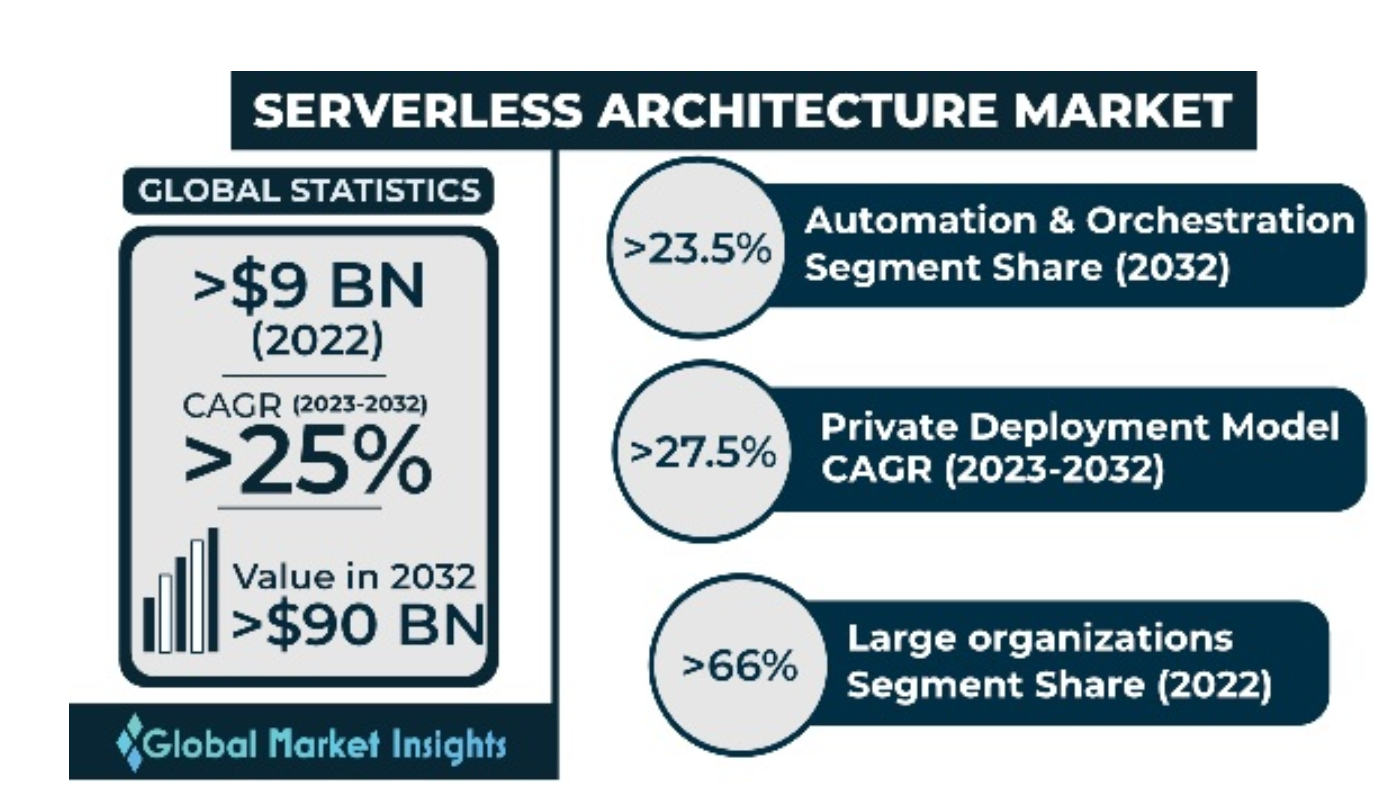
\includegraphics[width=0.5\linewidth]{images/Serverless-Arch-market.PNG}
    \caption{Serverless Global Market Share}
\end{figure}
\begin{flushright}
    - \cite{Global_Market_Insights_ID_GMI3796_2022}
\end{flushright}
\end{flushleft}
\pagebreak

\section{Serverless Framework}
\subsection{FAAS: Function As A Service}
\par
\begin{flushleft}
Function as a Service or FaaS is the basic building block of Serverless framework, (including AWS Lambda or Azure Function). 
\begin{quote}
\textit{Function as a service (FaaS) is a category of cloud computing services that provides a platform allowing customers to develop, run, and manage application functionalities without the complexity of building and maintaining the infrastructure typically associated with developing and launching an app.} \\
(\cite{Wiki_function_as_a_service})
\end{quote}

\par
In FaaS, the cloud vendors are responsible for providing and managing the complexity of related application server, infrastructure, frameworks, security, and everything that the application needs to execute a specific function in an application. 

\begin{quote}
\textit{
The “compute containers” executing your functions are ephemeral, with the FaaS provider creating and destroying them purely driven by runtime need. Most importantly, with FaaS the vendor handles all underlying resource provisioning and allocation—no cluster or VM management is required by the user at all.}\\ ( \cite{Roberts_Mike_2018} )
\end{quote}

Following FaaS approach Serverless offers on-demand functionality, which might live just for a single invocation. The cloud infrastructure will scale it to zero in preserve infrastructure and running costs. As such FaaS functionalities are opinionated stateless applications. This is a key difference between other architectural cloud-based offerings like containers and PaaS. 
 AWS Lambda is the first publicly cloud-based offering of FaaS or Serverless. 

\subsection{Functional Triggers}
FaaS functionalities are typically triggered by events. Event Types are defined by the vendors. The vendors for Serverless are also responsible in managing connections from various message sources. For Example:  Azure Functions can react to Messaging Sources like Event-Grid, Event-Hub, Blob Storage or simple HTTP triggers. This approach fits perfectly with Microservices patterns of keeping the application event-driven and asynchronous.

One important feature of Functional Trigger, offered by Serverless, is that the developers do not need to write any infrastructure or platform-related code in this application. The Serverless framework also manages the consumption of data and its conversion to the “Cloud Event” format.

FaaS, will not require any application server to up in running, it can be “Scaled to Zero” if there is no event triggered. This difference, as stated earlier my Mark Roberts, becomes a key factor in making FaaS solutions cost-effective. FaaS applications are booted and scaled up when an event is triggered from a configured event source.

However, the initial request in Faas has higher latency, (could be up to seconds,) than any other application platform. This “Cold restart” is an issue for FaaS and for Serverless offerings. The restart will depend on many factors, predominantly the application runtime and its runtime libraries. The effect of “cold restart” on the Quality of Service depends on type of traffic and applications. 

\subsection{Vendor Locking}
In cloud computing vendor lock-in is a problem when an organization adopts a specific could vendor find migration of application and data to alternative providers, extremely expensive and time-consuming. The cloud vendors' framework and their adoption in application make it incompatible with other vendors.
 The Vendor Lock-in occurs in various ways: 
 \begin{itemize}
     \item by designing a system incompatible with software developed by other vendors
     \item by using proprietary standards or closed architectures that lack interoperability with other applications
     \item by licensing the software under exclusive conditions
 \end{itemize}

 Vendor lock-in discourages organizations in adopting new and emerging cloud technologies like Serverless. There is no standardization of Serverless design, data structure and code that could favour an easy transition from one cloud vendor to other, without an expensive redesign of the entire application. 

 \begin{quote}
 \textit{
Existing cloud computing solutions for enterprises have not been built with interoperability and portability in mind, hence applications are usually restricted to a particular enterprise's cloud or a cloud service provider.}\\
\cite{Opara-Martins-2014}
\end{quote}
\par 
In reality, this claim is somewhat correct because existing cloud solutions are tightly coupled to the proprietary technology they were designed for, consequently, locking customers into a single cloud infrastructure, platform, or service preventing interoperability and portability of data or software created by them. 
\end{flushleft}
\section{Cloud Native approach for Serverless}
\begin{flushleft}
Cloud Native Computing Foundation (CNCF) introduced Kubernetes to counter vendor lock-in issues created by cloud vendors offering PaaS. Kubernetes is a new platform allowing containerized applications to run in their own sandbox (POD), isolated in their namespace.
Kubernetes is now accepted as the standard for PaaS. All major cloud vendors support the deployment of Kubernetes clusters in their cloud environments
\end{flushleft}
\section{Knative }
\begin{flushleft}
The knative project was started by Google in 2018, with the aim to facilitate the deployment of a Serverless application using Kubernetes. Knative offers Serverless features like Scale to Zero, auto scalability, abstraction from PaaS and Infrastructure, and use of the eventing framework.
Knative, leveraging from the underlying Kubernetes platform, offers a portable runtime and open API, which makes Serverless applications fully Cloud Native. This increases interoperability and eases the transfer of applications from existing cloud providers to others.
\begin{quote}
    \textit{Knative is an open-source initiative aiming to provide a platform for developing container applications on top of the Kubernetes container orchestration platform. It offers ready-to-use components built with Kubernetes Custom Resource Definitions (CRDs) for developers to build, deploy, and scale their functions end-to-end from source code.}\\
    \cite{lin2019mitigating}
\end{quote}

\subsection{Knative Function}
Knative provides the framework for creating a Cloud Native Serverless function that is deployed to a Kubernetes cluster. There are three components to Knative (a) Build, (b) Serving, (c) Eventing.

\textbf{Knative Build} component is responsible for converting the functional code to a container image, burning code or logic, the runtime, dependencies, configuration, and environment variable, etc. to OCI standard Image, pushing it to an internal Kubernetes registry.
\begin{figure}[h]
    \centering
    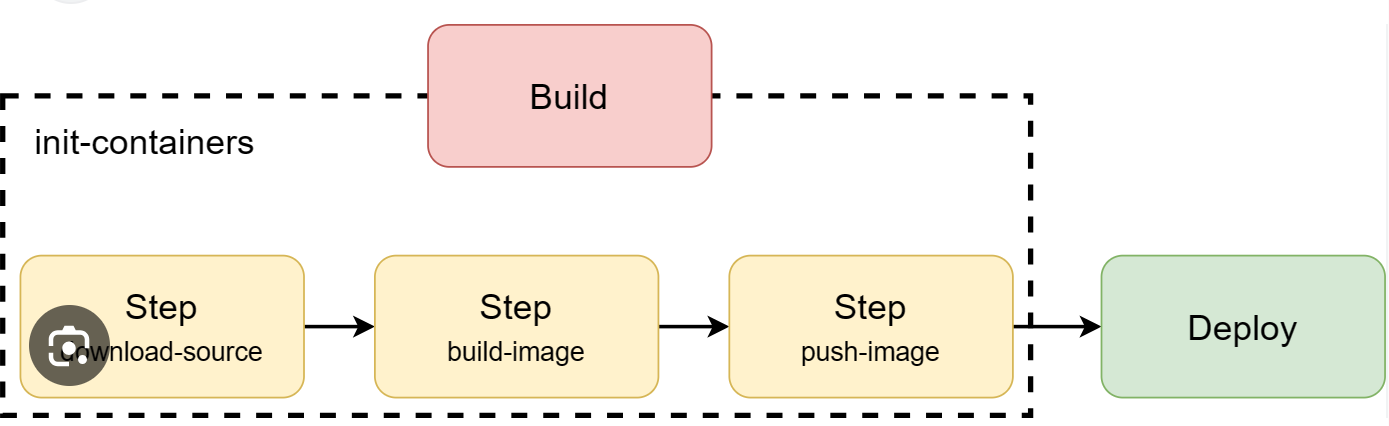
\includegraphics[width=0.5\linewidth]{images/knative-build.png}
    \caption{Knative Build Stage}
    
\end{figure}

\textbf{Knative Serving} is a request-driven provisioning component, responsible for auto-scaling Serverless containerized instances. It also takes care of load balancing. 
Knative Serving also abstracts the Kubernetes service to administer the provisioning of new service versions. It also manages configuration updates, by rolling out a new immutable revision representing the updated functional state. Each service saves specific routing information to redirect traffic to a specific instance version.
\begin{quote}
   \textit{Knative Serving is ideal for running your application services inside Kubernetes by providing a more simplified deployment syntax with automated scale-to-zero and scale-out based on HTTP load. The Knative platform will manage your service’s deployments, revisions, networking, and scaling.} \\
   \cite{Sutter_Sampath_2020}
\end{quote}
\par
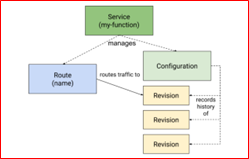
\includegraphics[]{images/knative-serving.png}

\subsection{Leveraging Service Mesh}
Knative leverage the service mesh to efficiently manage traffic routing between services which maintain immutable revision of Serverless application. It aids in satisfying the Serverless framework requirement of dynamic scaling, scale to zero and ease of deploying new versions. Various Service Mesh technologies are available that can be used in Knative example: Istio, kourier, etc.

\subsection{Knative Eventing}
Knative Eventing provides sets of primitives for consuming and producing events, assisting in satisfying the Serverless requirement of event-driven applications. 

\begin{quote}
\textit{Knative Eventing was to enable late binding of producers and consumers. It should be possible to connect consumers to producers without either component needing to know the configuration of the other.}
\end{quote}
\begin{flushright}
\cite{cncf_to_host_cloudevents_in_the_sandbox_2023}
\end{flushright}
 \hfill\break   
Just like any other message-driven system, the Knative Eventing component is composed of:
\begin{itemize}
    \item an Event-Source, which produces events from various sources.
    \item a Channel, which saves and buffers the event between and producers and consumers.
    \item 	and Subscriptions, which forwards events from Channel to services or other channels
\end{itemize}
\begin{quote}
\begin{figure}[h]
    \centering
    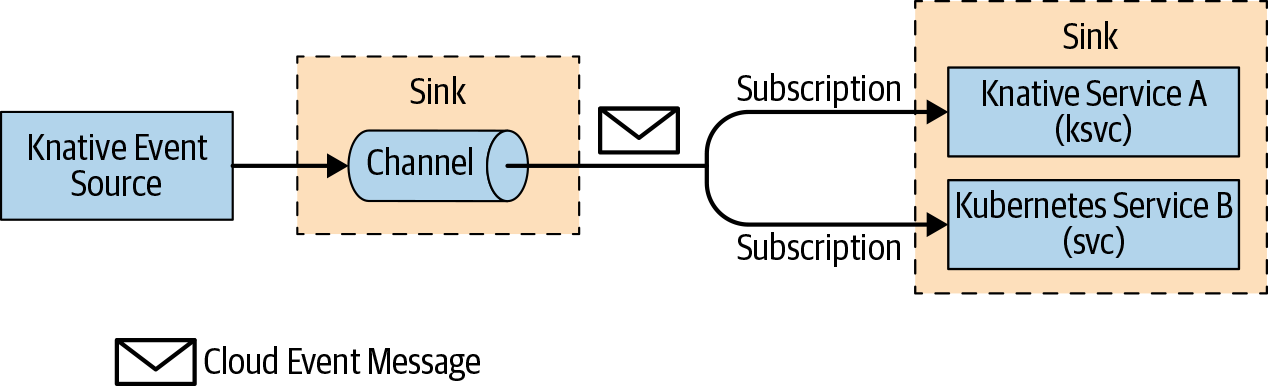
\includegraphics[width=0.5\linewidth]{images/knative-event-channel.png}
    \caption{Knative Eventing Channel,  Ref: \cite{Sutter_Sampath_2020}}
    \end{figure}
\end{quote}

The message-driven approach makes services loosely coupled and independent. Knative eventing framework makes Serverless applications event-driven and asynchronous. Knative being open source also allows the plugging of third-party Event Sources like Kafka Topics. 

The developers leverage for Knative API and Eventing platform to consume events in their functional code without writing any infrastructure code for consuming and parsing it. The API makes it possible to consume events in the standard “CloudEvent” format. 
\end{flushleft}
\section{Azure Function}
\begin{flushleft}
\textbf{Azure Function} is a Serverless offering by Microsoft. It allows developers to deploy their FaaS application on Azure Cloud using a Pay-as-you-go model. It followed all the features of Serverless, like the scale to zero, horizontal scalability, complete abstraction from the Platform, and eventing framework. It offers SDK and CLI to build and Deploy Serverless applications to the cloud, using various programming languages and frameworks like Java, .Net, NodeJS, etc.

Azure Functions adopts the Azure Eventing framework to provide a comprehensive set of event-driven triggers and bindings. This binding connects Azure functions to other services without having to write extra code. This provides the capability of Azure function to be asynchronous and event-driven, without worrying about platforms and infrastructure.

Azure deploys functions (or FaaS) application, its code, runtime dependencies and configuration information with the application file system associated with a Storage account. This allows Azure function runtime to access and execute code when the function is triggered. 

\subsection{Azure Eventing}
Azure Functions leverages Azure eventing framework to create Event-Driven, Asynchronous Serverless Functions. The common use case for this feature is creating Workflow. 
\begin{quote}
    \textit{Serverless is a great fit for event-driven architectures because each message acts an individual independent unit of work that can be processed Serverlessly.} \cite{ANDERSON_2024}
\end{quote}

Azure Eventing framework supports event-sourcing and event-subscription. Azure Serverless framework consumes events from the Eventing Channel, triggers, and routes it to the Functional instances. If the instance is scaled to Zero, an instance is restarted. Azure Serverless framework abstracts all infrastructure and platform complexity from the code, making the function API consume CloudEvent formatted data. The configuration also allows the Azure function to push data back to the Event Channel.

\begin{quote}
    \textit{CloudEvents, an industry initiative that members of the CNCF Serverless Working Group contribute to, provides a consistent set of metadata to make events easier to work with for publishers, middleware, subscribers, and applications.} 
 \cite{cncf_to_host_cloudevents_in_the_sandbox_2023} 
\end{quote}


\subsubsection{Three Patterns of Knative Eventing}
\begin{itemize}
    \item Source To Sink: It is a very basic connection between the Event Source to service that receives the event unconditionally (or SINK). There is no support for filtering, queueing, etc.

    \item	Channel and Subscription: Knative defines a Channel and subscribes it to other backend messaging services like In-Memory, Kafka, etc. for event sourcing. Each message in the channel is in CloudEvents format. There is no message filtering in the Channel.

    \item Triggers and Broker: Knative creates an Event Channel from the Broker, and the Trigger creates a subscription applying filter. These filters are based on CloudEvents attributes, are applied before it is dispatched to the configured Sink.
\end{itemize}

\subsection{Building and Deploying Function in Azure}
Azure SDK and CLI provide templates for creating Azure Functions. Developers can choose the programming language and type of event triggers. There are additional manifest files that contain event bindings and configs. 

Azure CLI builds the Azure function and publishes it to Azure Functional Application. The process of publishing will archive the package and do a remote build of the package. The process will then sync the function with the Event Trigger. The function will remain in a dormant state (i.e. scaled to zero). The function performs a “Cold Start” when the event is triggered. Deployment to Azure Function App, automatically connects it with Azure Application Insights, collecting metrics for monitoring.

Automation of deployment can be achieved using CI/CD and storing the application to GitHub. 

\subsection{Cold Start}
Cold Start is a term used to represent the phenomenon that applications that is not in a running state, will take a longer startup time. As such it will increase latency in processing data if there is no running instance. The startup delay is influenced by various factors including bootstrapping application runtime, code and its libraries. This bootstrapping startup delay is also witnessed when Auto-Scalar provisions instances to support the traffic. This initialization time is unavoidable and lasts until the application starts responding. Depending on the application use case, this latency caused by Cold-start can create a backlog and time-outs.

\section{Deployment overhead of Knative}
Azure Serverless Platform provides all the application framework needed to build, deploy, and run a Serverless application. Developers can use Azure Portal to create a Functional Application, then can use CLI or CI/CD to push Image. Azure Portal also allows developers to configure Serverless applications, set up environment variables, create connectivity etc. 

Knative is offered over Kubernetes. It is deployed as CRDs and set of application POD and Services on the Kubernetes cluster. These are the required components that must be deployed before deploying any FaaS.
\begin{itemize}
    \item Istio (Service Mesh): It enables secure service-to-service communication and authorization, using sidecars processing secure communication controlled by a central plane. 
The deployment contains set of CRDs, Services, Gateway components etc.
    \item Knative Serving:  Manages deployment, configuration, revision and routing of the Knative application in Kubernetes.
    \item Knative Build: The Knative Build framework is read the Function code and manifest, to prepare a container image, pushing it to the Container Registry.
    \item Knative Eventing: Knative Eventing provides the framework and API to configure and integrate Messaging Channels, Brokers, and Triggers. It facilitates the integration of third-party message brokers like Apache Kafka and Rabbit MQ as event sources.
\end{itemize}

Knative offers these services as a set of CRDs and Kubernetes Services. Knative provides the deployment YAML file to configure and deploy these services and CRDs. 

The initial deployment of Knative frameworks and components offers complexity and expert understanding of Kubernetes and Knative functioning. However, these steps can be considered as One of the Admin jobs, automated using CI jobs. The controlled deployment using the YAML configuration file offers greater control and flexibility in preparing the Serverless Infrastructure.
Since the Knative framework requires many mandatory components and services to be deployed and running, it increased the physical hardware requirement of the Kubernetes Nodes to a minimum of “Standard D2 V2” (, which is 4 Core CPU and 14 GB Ram). 

\subsection{Deploying Functional Service in Knative}
Knative CLI creates a template project for its Function, using the template and building a pack of choice. The template also allows the option to choose the event type which can be either HTTP Trigger or CloudEvent. 
Knative CLI, creates a startup project, with basic configuration creating an empty function code, manifest files and build files. Users can place business logic to the function code, consuming the CloudEvent or HttpRequest body. All Event Sink and Event Source must be configured beforehand using the config YAML file.
Knative provides CLI to build and deploy the Knative Function as an OCI container image file. It compiles all the dependencies and runtime. The deployment process also deploys a Knative Service to the Kubernetes cluster. The container image is pushed to the container registry which is accessed by the Kubernetes service. The Function is now deployed to the Kubernetes cluster and is now accessible for external web requests. Redeployment of function will update the container image and the Service running in Kubernetes Cluster. The Knative Serving will route traffic to the new image version. 
CI/CD pipeline can streamline the build and deployment of Knative functions and services. It will leverage the Knative Build and CLI under the hood to deploy or update Function to the cluster.

\section{Developing and Event Driven Application}
Developing an event-driven application using Azure Function and Eventing framework is simple and painless, compared to Knative.
\hfill \break
For event-driven application using Azure Function, a trigger is created that subscribe to specific events in EventGrid, EventHub or other Channels. The trigger is configured to invoke an Azure Function when the event is received. Trigger also supports the filtering of events. 
Azure Portal allows developers to create and configure these triggers from Event Grids or Event Hub.
Azure CLI creates a skeleton functional code file and configuration file. User can place their business logic in the functional code file. The configuration file contains the Bindings for the event subscription. These Bindings are for both, the input and output of events from Azure Function. 
\hfill \break
A Knative Event Trigger listens to CloudEvent from Broker and dispatches it to a SINK, which will be a Knative Function. In the same way, a source binding is created to “Event Source” from Knative Function to Event Broker. Knative Trigger also has the option to specify a filter so that it can listen to specific types of events.


\section{Workflow Orchestration }
Both Azure Function and Knative provide options to create a Workflow. These workflows are created using Eventing Framework which includes Event Source, Sink, Event Brokers, and Triggers. 
\hfill \break
The workflow orchestration consumes events from the message broker and triggers events that are invoked Serverless. The result of invocation will transform of message data received as CloudEvent and pass to the next stage. 
\hfill \break
There are 2 types of Workflows created in Knative 
\begin{itemize}
    \item Parallel
    \item Sequence
\end{itemize}
\textbf{Parallel Workflow}, offered by Knative is a set of CRD that defines a set of branches. Each branch contains filters and subscriptions. Knative Workflows creates channels and Subscriptions under the hood. Both Filter and Subscription refer to a Knative Service Function.
\hfill \break
\textbf{Sequence Workflow}, offered by Knative is also a set of CRD that defines an order list of functions that must be invoked. Each step creates a filter and transforms events as they are passed. Knative Sequence workflows also create Channels and Subscriptions under the hood.

\section{Sample Use-Case}
A sample Use Case of the work flow showing an Invoice Management System, which will demonstrate small Event Driven Microservices. A typical Invoice Management system involves Client Generating Invoice, Invoice is registered, then Payment is made, Invoice is Validated and Audited. All these stages will require unique Serverless, Event Driven Microservices. The Status and Type of Invoice will act as filter for different Microservices to react. A Broker and trigger design with filter is a better approach.

We have 2 code bases one for Azure another for Knative. Both involves CloudEvent as intermediate data structure. The Logical code is same for Knative and Azure. Deployment process will be different. 

\subsection{Application Code base}
\textbf{Azure Function:}\\
https://github.com/AINULX00159358/InvoiceManagerAzure \\
\textbf{Knative Code base}\\ 
https://github.com/AINULX00159358/InvoiceMgrKnative\\
\textbf{Test Scheduler code base}\\ https://github.com/AINULX00159358/InvoiceMgrTestScheduler\\
\pagebreak
\subsubsection{Using Broker and Triggers}
Both Knative and Azure Functions supports Event Channels with Broker and Trigger subscription.
Broker is just a facade or over Channels, facilitating substitution of channel without modifying the subscription and triggers.
Triggers facilitate event subscription, with Filters and a Sink. The Sink is a Serverless Function which is activated in response to event trigger.
The downstream Sink service supports a CloudEvent response, which is routed back to the Broker, and finally to event channel. 
\begin{figure}[h]
    \centering
    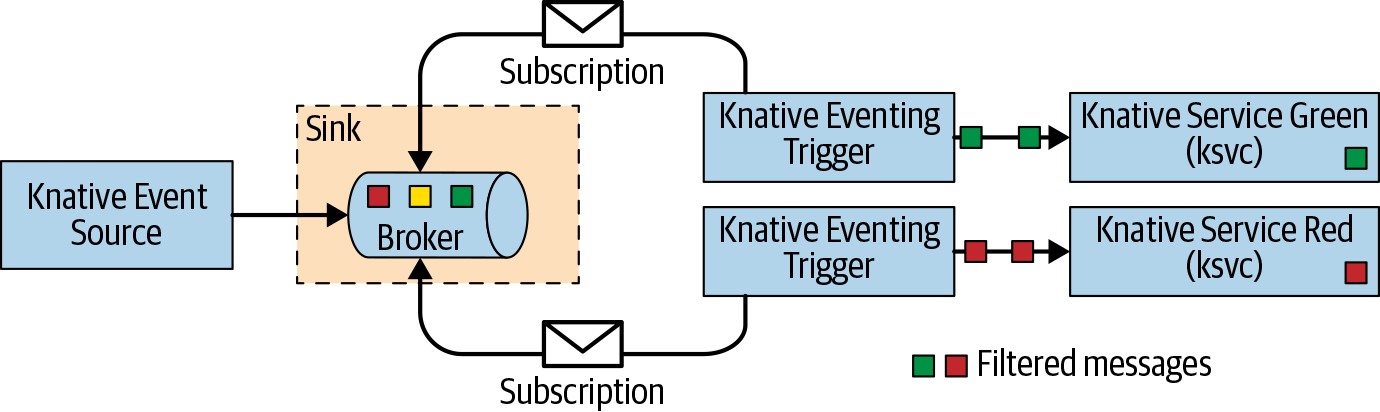
\includegraphics[width=1.00\linewidth]{images/knative-event-broker.png}
    \caption{Knative Event Source, Broker Trigger and Sink}
    \textit{
    Ref: \cite{Sutter_Sampath_2020}}

\end{figure}


\subsection{Application Design}
Application is design using cluster of Microservices, deployed as a Serverless Application. 
Application will be subscribed to the Broker by configuration.

Application maintains the Status of the Invoice which is updated during each steps, and also acts as a filter.

The Status of the Invoice will update from Unknown -> New -> Pending -> Paid -> Closed

A Test Scheduler is deployed as Simple Kubernetes Pod, which will start Injecting dummy client Invoice Request to the Broker Endpoint. Code can push data at various TPS like 30, 60, 100 etc.


\section{Analysis}
\subsection{Deployment}
Knative has an overhead of setting up the Kubernetes cluster, Service Mesh and Knative Infrastructure. In production environment a reliable messaging infrastructure like Kafka must be deployed.

Infrastructure cost of setting a proper Knative environment which can support high traffic bandwidth, messaging infrastructure and scalibility of Serverless will require provisioning of large capacity nodes.

\subsection{DevOps overhead}
The Knative code must be converted and pushed as docker image to the container registry. 
Kubernetes POD will pull the container image from the registry. This will effecting "Cold Start" of the POD. 
The Image Pull Policy might not always be set to "IfNotPresent" due to security implication in some companies. 

In Azure the function build, do not convert the code to a docker image, instead it stores the function files in its file system.

\subsection{Knative Cold Restart}
Knative provisions a FaaS just like Kubernetes  provisions Applications with PODS. PODs for are applications is orchestrated by Kubernetes to match the SLA. Knative instructs the Kube API in provisioning the Serverless , and scale it zero.  

Just like any application provisioning in Kubernetes, Kube API will first download docker image, worker node will prepare the image mounting physical resource, followed by provisioning the Container. 
The container is started by loading Application runtime, which is followed by application initialization and finally the POD is made ready. The POD is now running state, with the Serverless function inside the application runtime. 

There are different distinct stages of execution leading to provisioning of the POD. 
\newline
\textbf{Cold Start:} When the application is being started for the first time
\newline
\textbf{Warm Disk Start:} When the docker image is already cached. The process starts from mounting of image, starting the container, application runtime and pods
\newline
\textbf{Warm Memory Start:} The container is resumed from the paused state. The costly, time consuming process of image pull, mounting and starting of container is avoided, thus speeding up the startup time.
\newline
\textbf{Warm CPU start:} In this case the container is already running as such the only latency that will apply will be the time application takes to respond to the request. In this is a case application was not scaled to zero.

\begin{figure}[h]
    \centering
    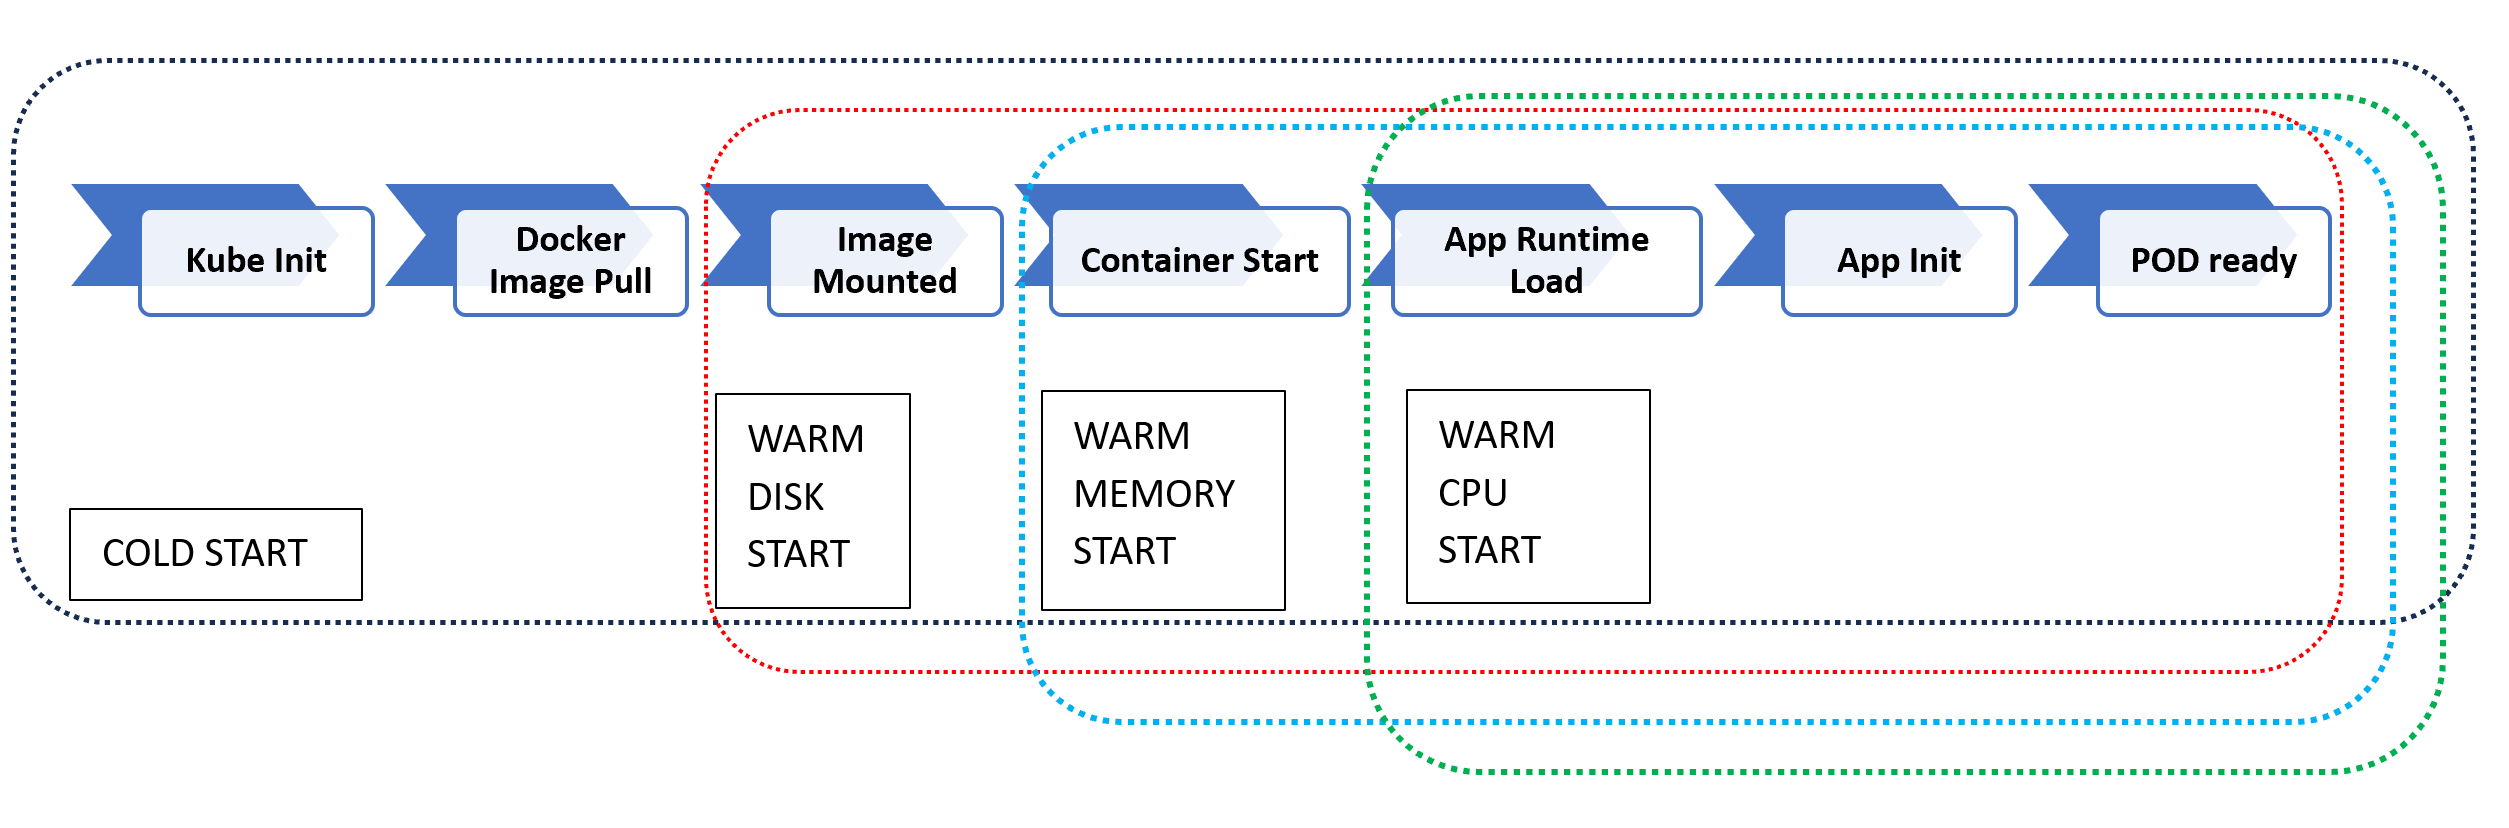
\includegraphics[width=1.0\linewidth]{images/Knative_lifecycle.PNG}
    \caption{Enter Caption}
    \label{fig:enter-label}
\end{figure}

\subsubsection{Metrics Recorded for Knative Application}

\begin{figure}[h]
    \centering
    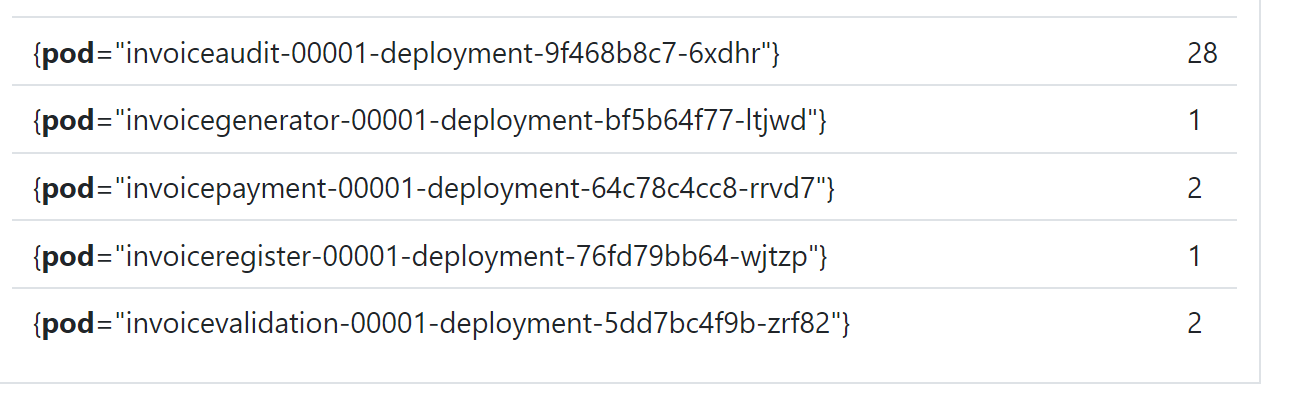
\includegraphics[width=1.0\linewidth]{images/ColdStart_prometheus.PNG}
    \caption{Enter Caption}
    \label{fig:enter-label}
\end{figure}

The metrics is collected by taking a delta of time in Seconds when POD is scheduled and achieved a ready state. 
This metrics is collected after Initial Deployment. In this case the 'Image Pull Policy' is set to IfNotPresent, which avoids pulling image from docker registry.
The deployment still time and consideration for creation of services and service-proxy, registration of public endpoints to registry.
This stage can be considered as Warm Disk start.

\begin{figure}[h]
    \centering
    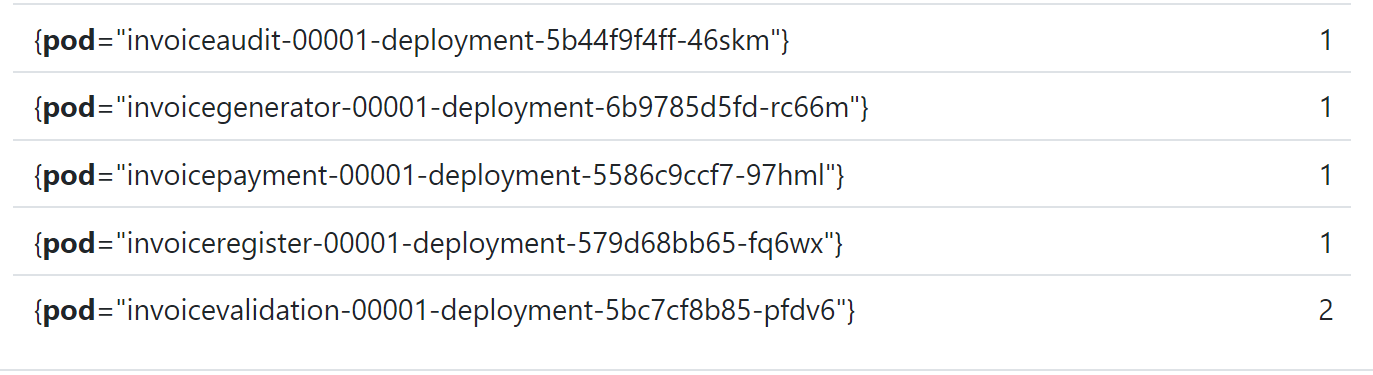
\includegraphics[width=1.0\linewidth]{images/ColdStartScaling-FirstTraffic.PNG}
    \caption{Enter Caption}
    \label{fig:enter-label}
\end{figure}
This metrics is collected after sending first Traffic, causing the Pods to Scale from Zero to One. This is the stage of "Warm Memory Start". Application is faster to start avoiding cost of Adrress registration etc. 

\begin{figure}[h]
    \centering
    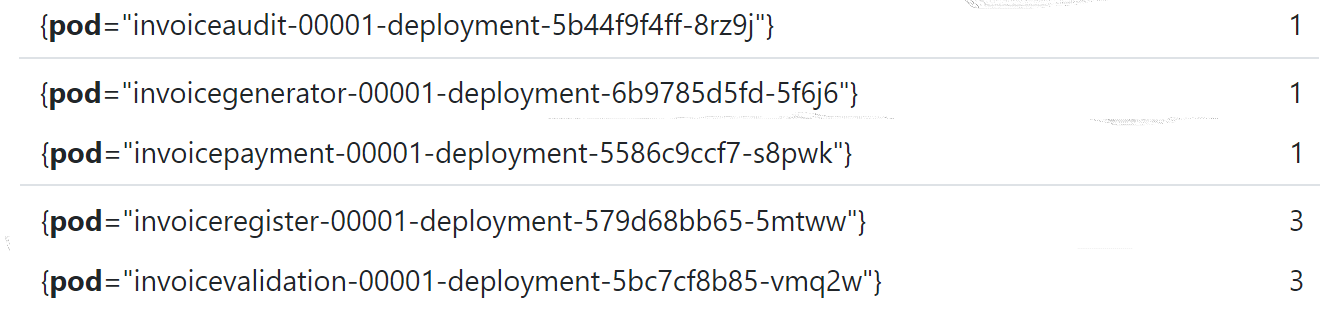
\includegraphics[width=1.0\linewidth]{images/Pods_Scaled-After-HighTrafficBust.png}
    \caption{Enter Caption}
    \label{fig:enter-label}
\end{figure}
This metrics is collected after traffic bust, which triggers auto-scaling. Traffic Bust challenged the capacity and capability of Current Kubernetes nodes, triggering scaling of pods. 
\pagebreak
\subsubsection{Autoscaling in Knative}

\quote{
\begin{figure}[h]
    \centering
    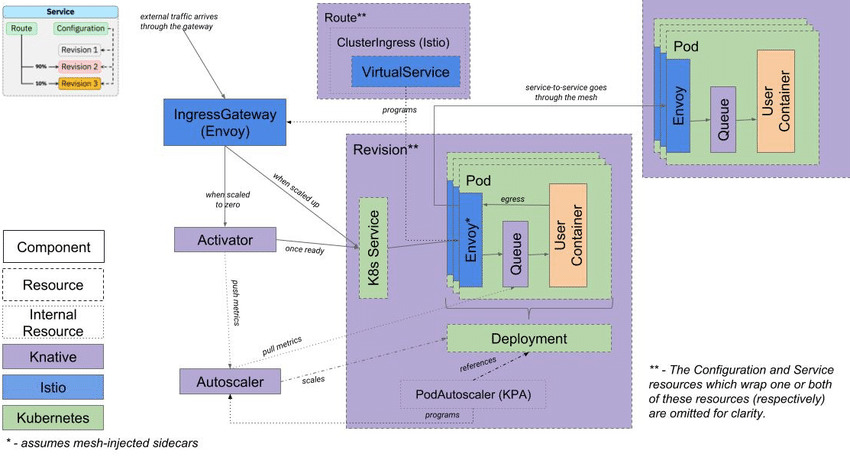
\includegraphics[width=1.0\linewidth]{images/Knative-Serving-Architecture.jpg}
    \caption{Knative Service Architecture }
    \cite{Towards_Serverless_as_Commodity}
    \label{fig:enter-label}
\end{figure}
}

This figure explains the full process of Autoscaling in Knative Serving Infrastructure.

The interesting case is when scaling from Zero to One:
\begin{itemize}
\item  Traffic comes to Ingress Gateway, then to the Serverless Services.
\item since the Pods are scaled to zero, requests are routed to the Activator. (i.e. Inactive Case).
\item Activator passes metrics to Autoscaler which obliged for scaling up the Pods, (from zero to 1).
\item Activator calls Knative Serving Deployment to spin up a pod, with all its containers and sidecars. 
\item Pod's cluster IP is now updated in Serverless Services.
\item Once Pods are scaled above zero, Serverless Services updates the Route, disconnecting the Autoscaler. The traffic is now routed directly to Pod's service Proxy.
\item The Knative Pod's sidecars and Envoy provide metrics which is now scared to Autoscaler directly, so that it can now decide to need to scale further based on incoming traffic.
\end{itemize}
\begin{quote}
    \begin{figure}[h]
    \centering
    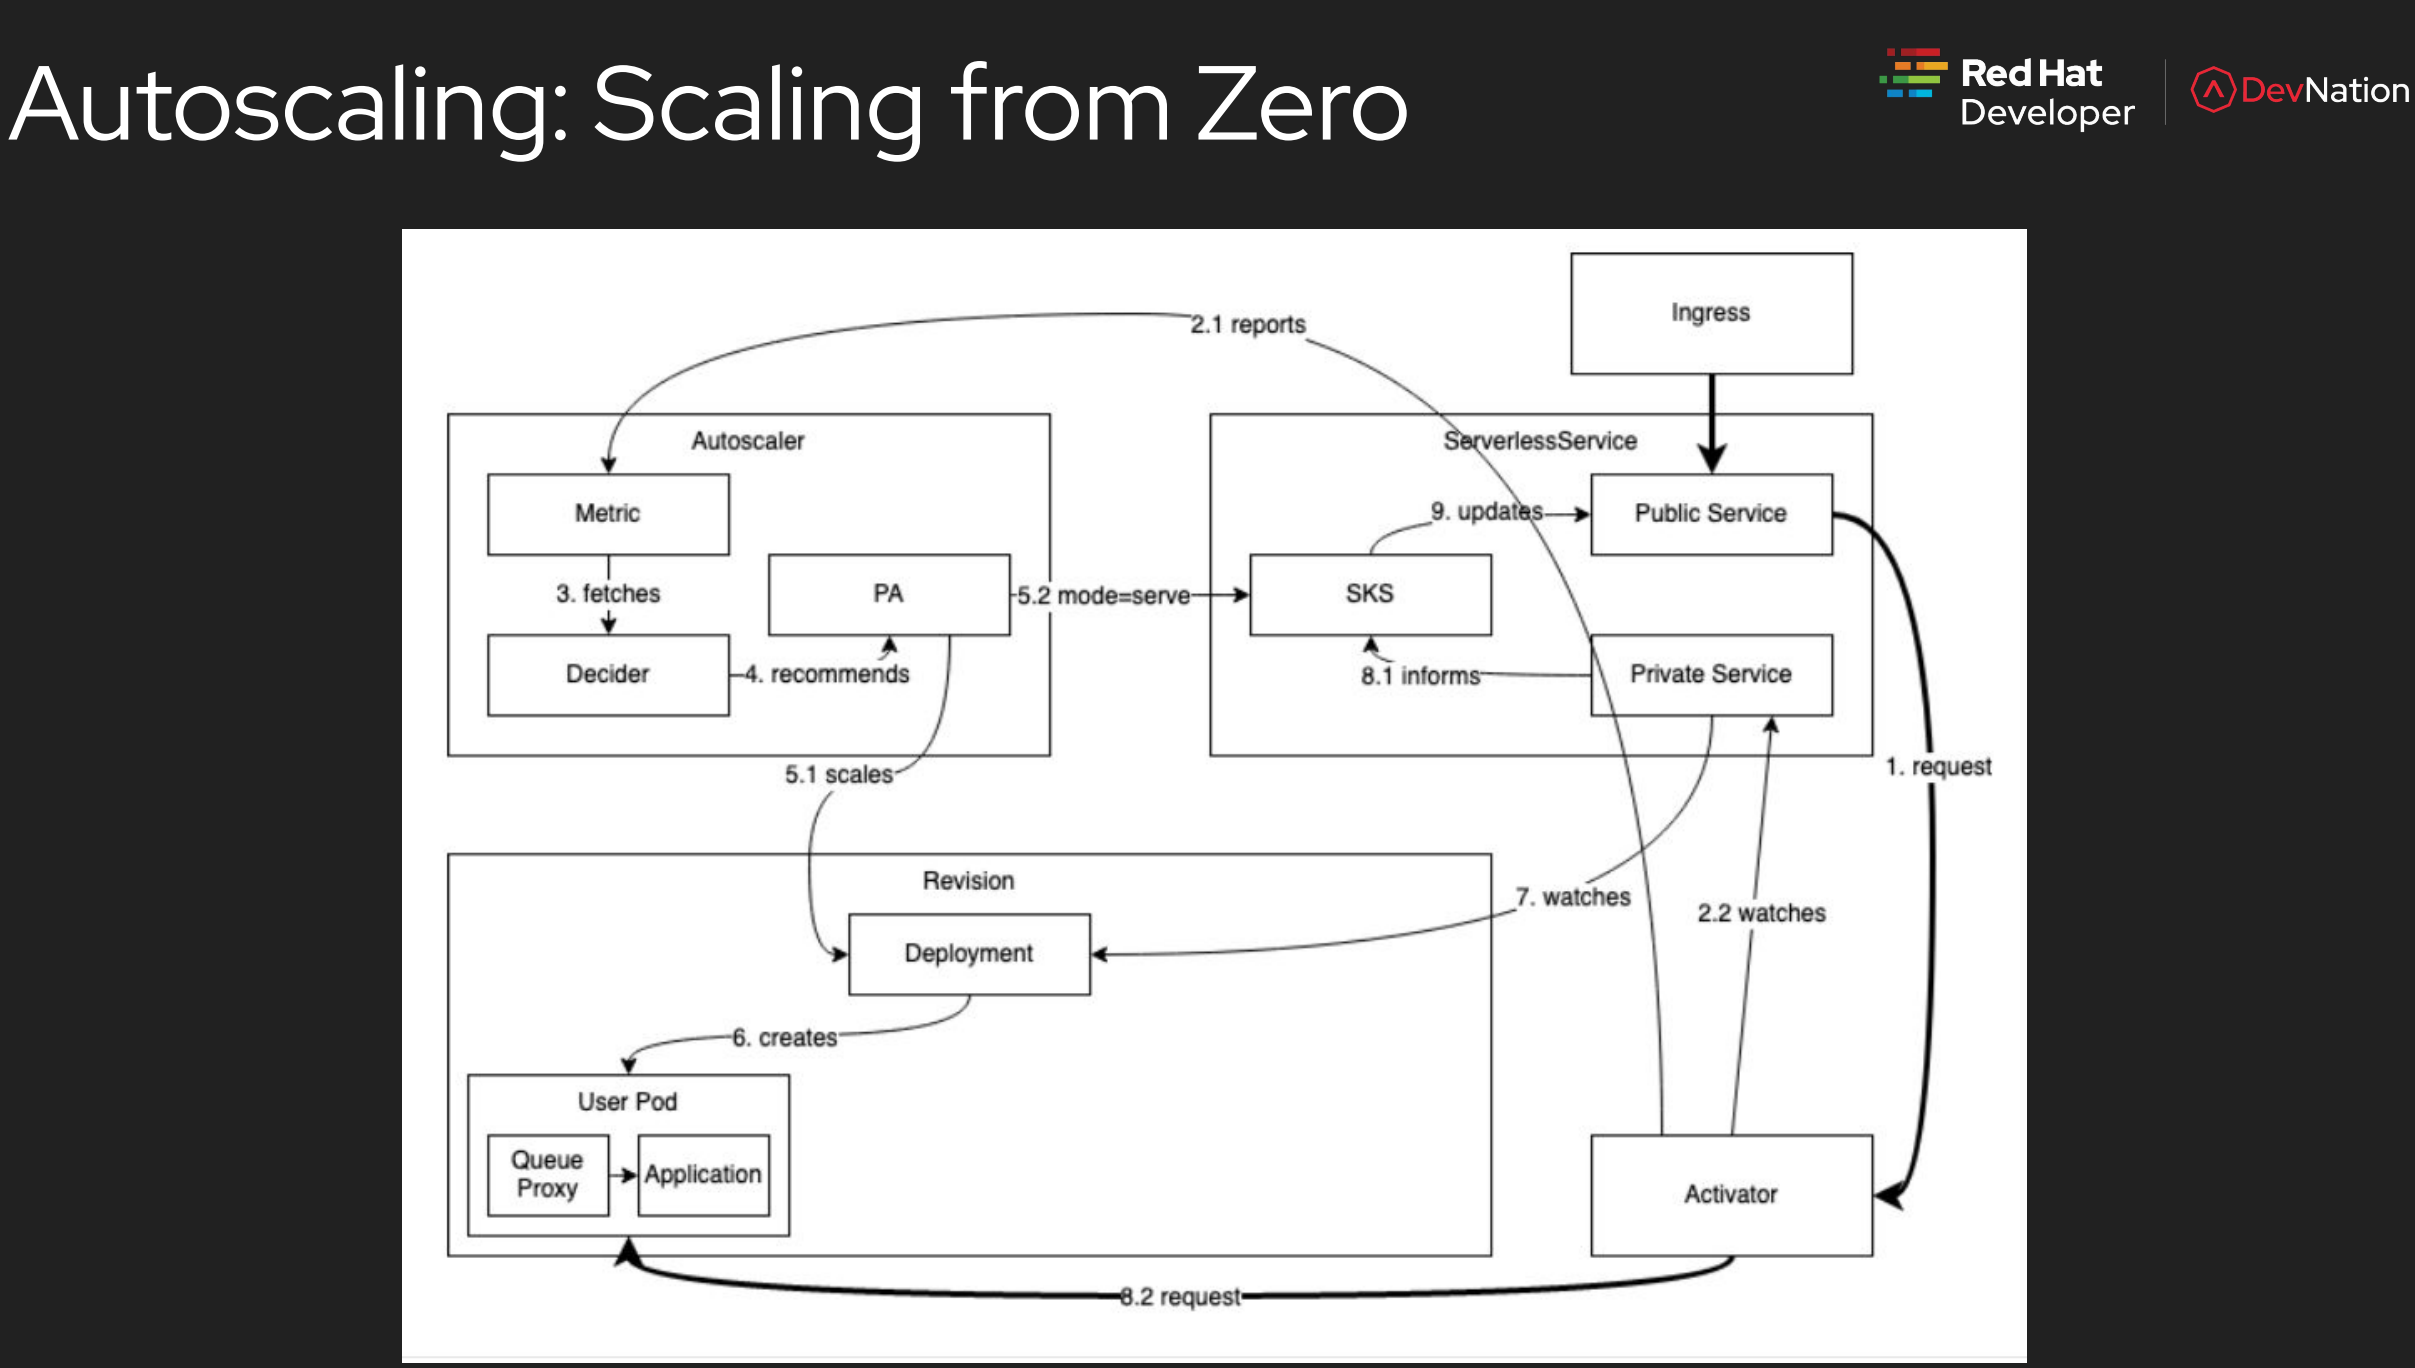
\includegraphics[width=0.5\linewidth]
    {images/KnativeAutoscaler-1.PNG}
    \caption{Autoscaler : Cold Start Case, Zero to One}
\end{figure}
\begin{figure}[h]
    \centering
    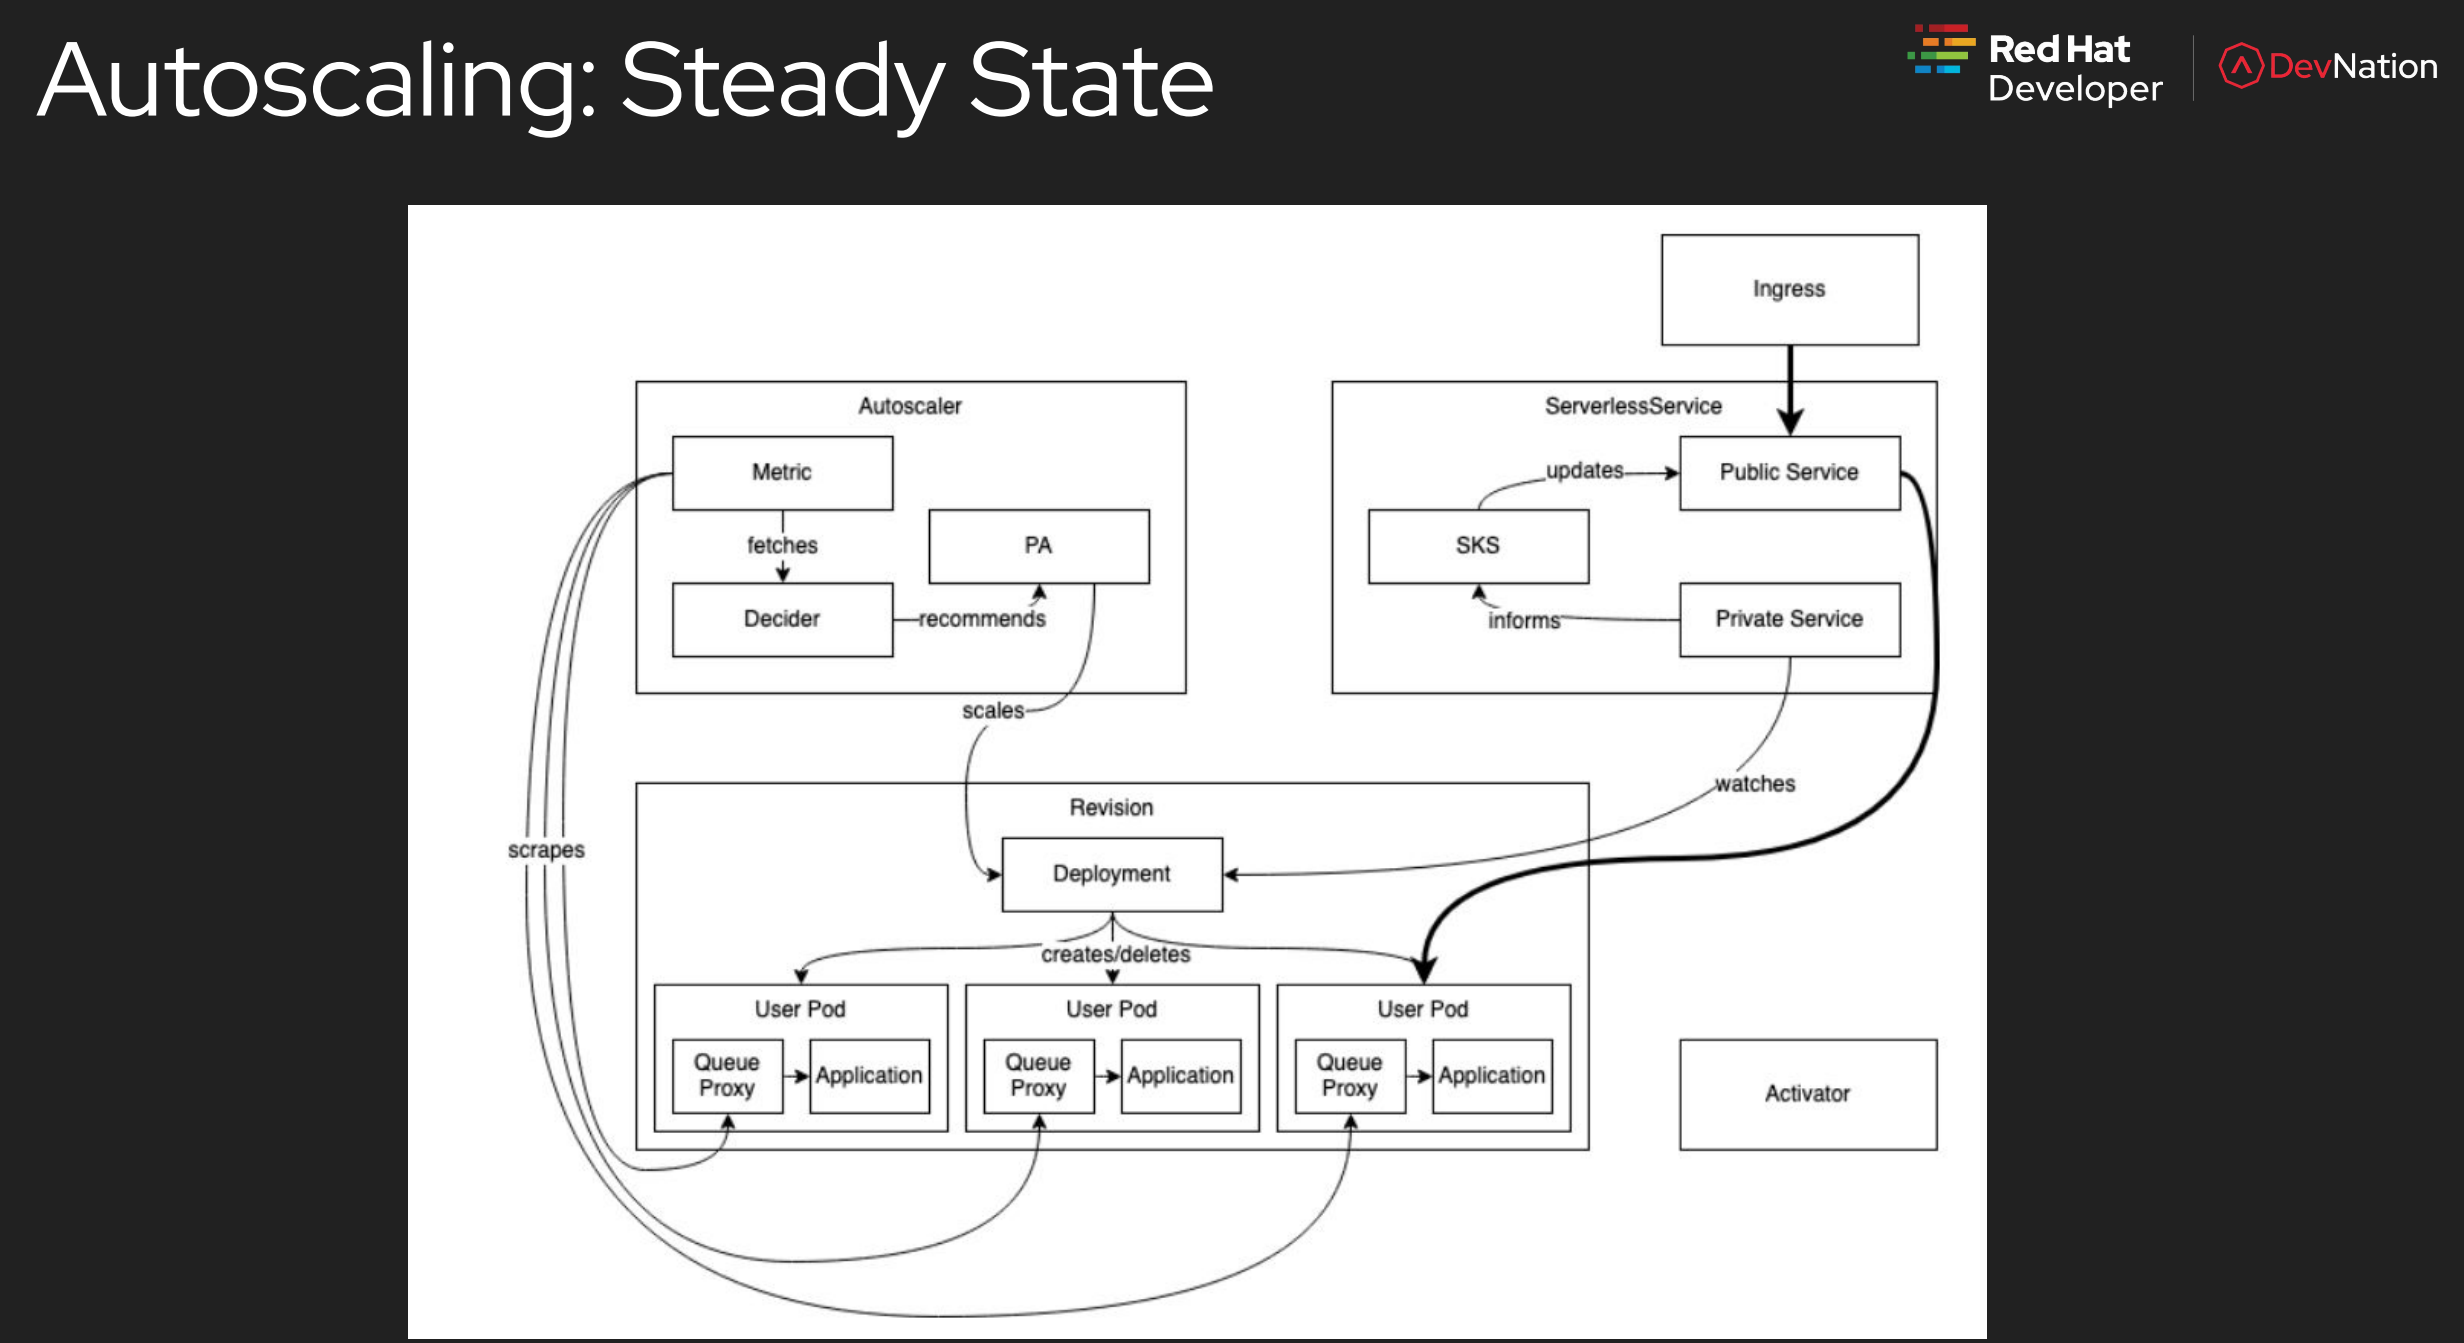
\includegraphics[width=0.5\linewidth]{images/KnativeAutoscaler-2.PNG}
    \caption{Autoscaler : for Normal Traffic }
\end{figure}
\begin{flushright} ref: \textit{\cite{Morie_2020}} \end{flushright}
\end{quote}

\newpage
\subsection{Azure Cold Start}
Azure Function store the functional code as file system in Azure Storage. When function needs to be executed Azure will allocate the function application to a server which should have capacity and capability to to execute it. The server also downloads and starts the the functional runtime. The Server is now ready to execute the functional code. 
\newline
The process of allocation of server to running functional runtime can consume more time depending on how it is configured, which can increase the overall startup time of functional application, adding to initial latency.
\newline
Azure handles this issue by keeping a pool of server in a "warm state", and drawing these servers as "workers" from pool. At any point of time, there are servers in the pool which are idle and pre-configured with Configuration and Functional runtime in a ready and running state. This feature is only available in Azure's Premium Plan.
\newline
When execution of function is triggered by incoming traffic:
\begin{itemize}
    \item Azure will allocate a pre-configured server from the pool. The server already has a functional runtime and configuration on it.
    \item After allocation, the server re-configures the functional runtime based on the application requirements.
    \item The Server now resets the Functional runtime and load any required extensions, using the \textit{function.json} file, specified the application manifest.
    \item In the last stage the Function is now loaded into memory and executed. Time take to complete the last stage depends on language used, size of application etc. The function is now in a ready state serving request.
\end{itemize}
\hfill \break
\begin{flushright}    
\begin{quote}
    \textit{"Making these 'pre-warmed sites' happen has given us measurable improvements on our cold start times. Things are now on the order of three to four times faster" 
 - \cite{Understanding_serverless_cold_start_2018} }
\end{quote}
 \end{flushright}



\begin{figure}[h]
    \centering
    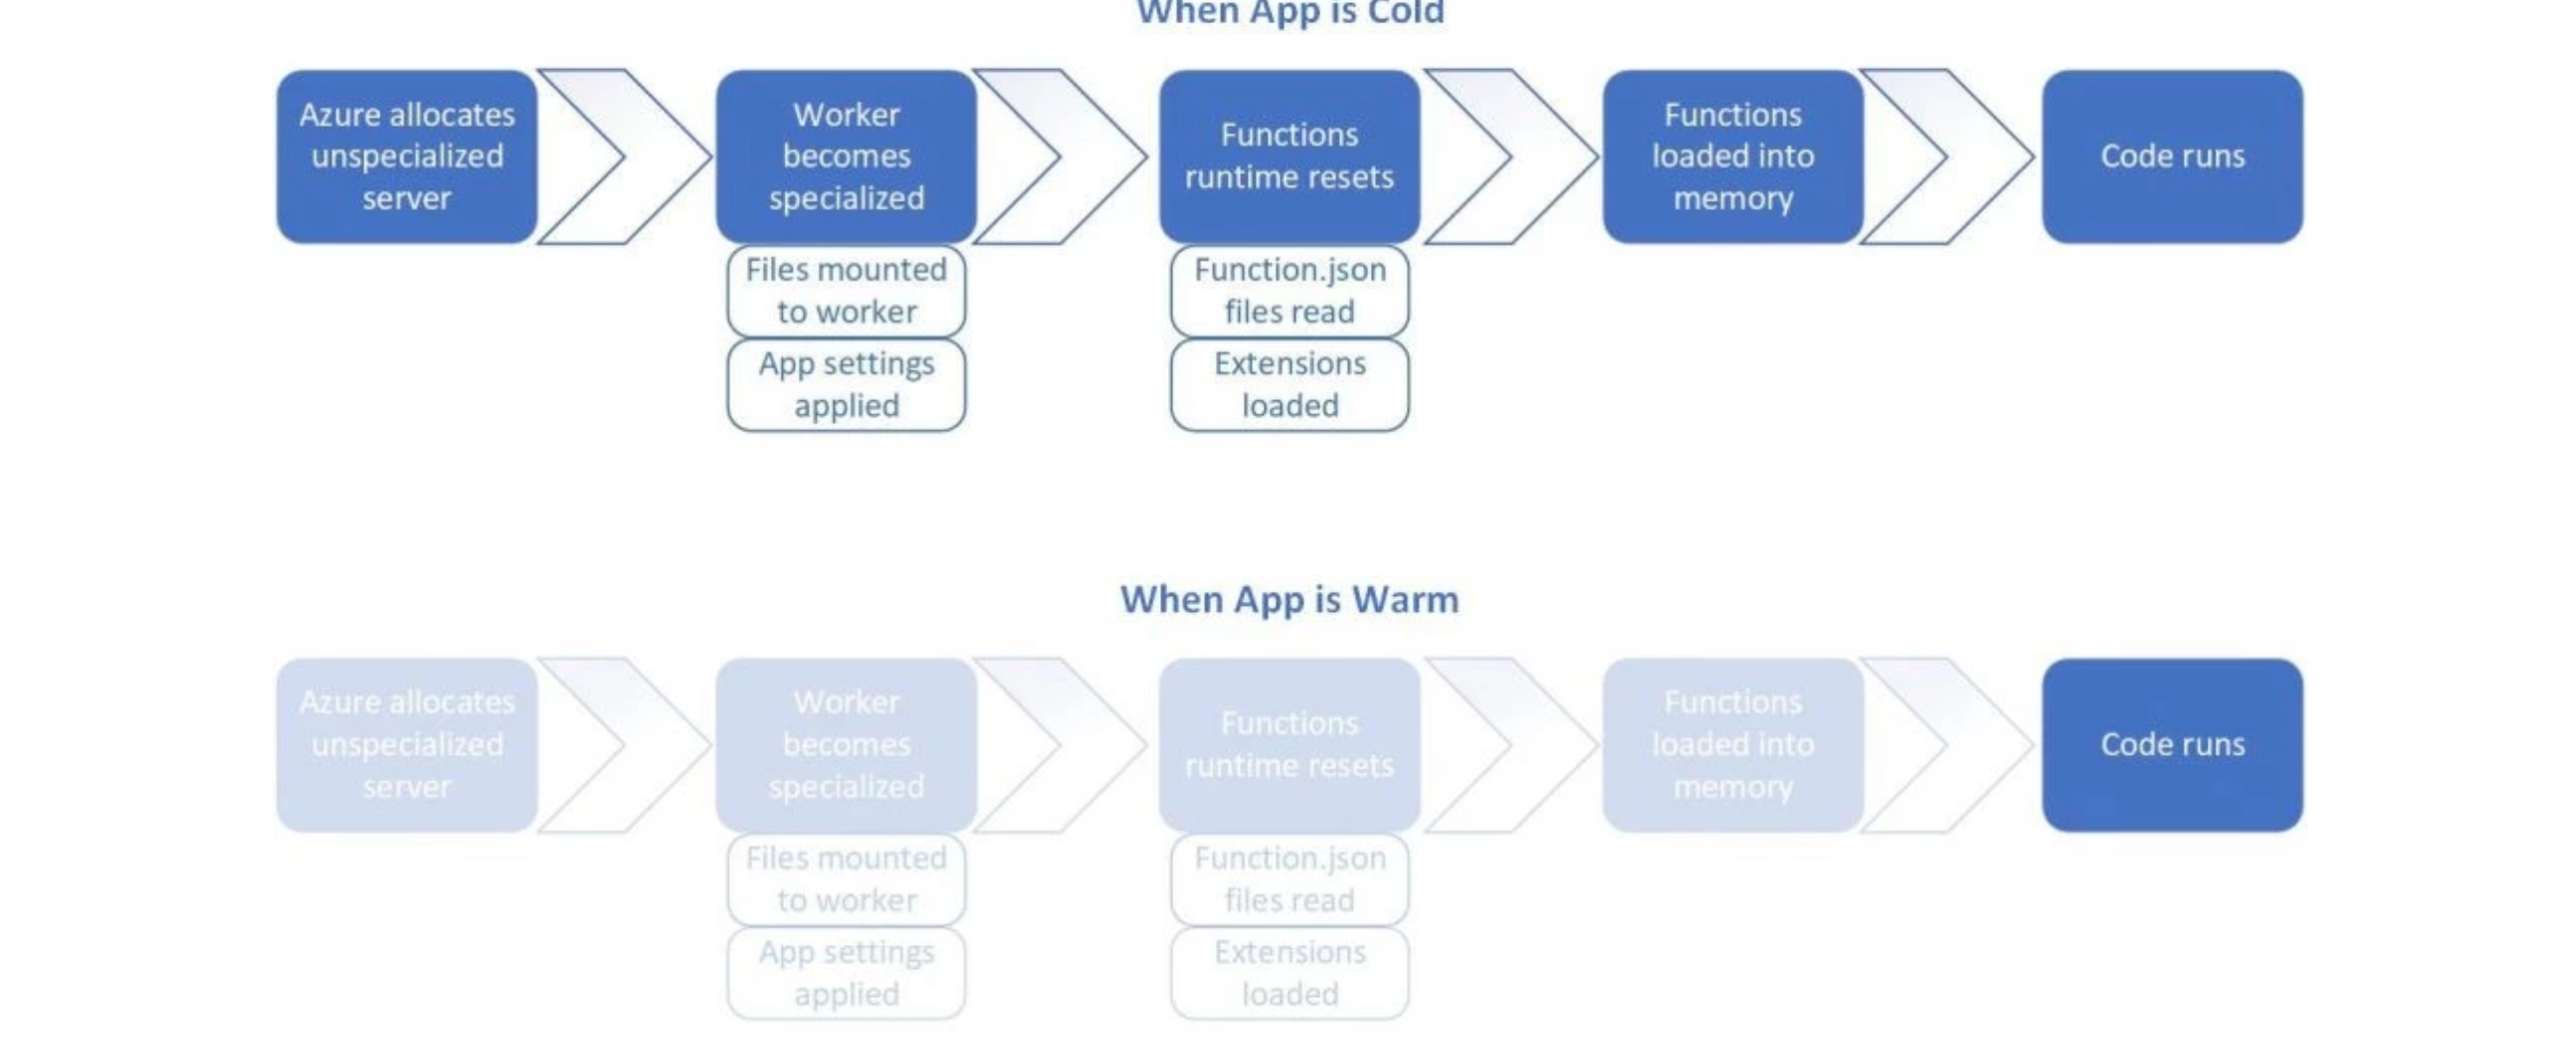
\includegraphics[width=1.0\linewidth]{images/Azure_lifecycle.PNG}
    \caption{Knative Lifecycle}
        Ref: \cite{Understanding_serverless_cold_start_2018}
\end{figure}
\textbf{Basic Consumption plan}
The Basic Azure Plan for Serverless hosting is "Consumption Plan". The Consumption plan scales application on traffic load factor. Customers are charged based on the compute resources utilized. The Compute instances for Functions hosts are dynamically added and removed based on the traffic load factor.

There is no support for Dockerized environment under Consumption plan

There are different Hosting Options available in Azure 
\begin{itemize}
    \item ASE : Azure Service Environment, which has high degree of isolation and scalibility.
    \item Azure Container Apps: Managed environment Azure Kubernetes Service (AKS) to run a containerized application using Serverless platform. 
    \item Kubernetes : As isolated and dedicated environment, running on Kubernetes platform.   
\end{itemize}


\end{flushleft}
\pagebreak
\newpage
\section{Conclusion}


\pagebreak
%prints bibliography from bibliography file.
\printbibliography
\end{document}